% CVPR 2025 Paper Template; see https://github.com/cvpr-org/author-kit

\documentclass[10pt,twocolumn,letterpaper]{article}

%%%%%%%%% PAPER TYPE  - PLEASE UPDATE FOR FINAL VERSION
 \usepackage{cvpr}              % To produce the CAMERA-READY version
%\usepackage[review]{cvpr}      % To produce the REVIEW version
% \usepackage[pagenumbers]{cvpr} % To force page numbers, e.g. for an arXiv version

% Import additional packages in the preamble file, before hyperref
%
% --- inline annotations
%
\newcommand{\red}[1]{{\color{red}#1}}
\newcommand{\todo}[1]{{\color{red}#1}}
\newcommand{\TODO}[1]{\textbf{\color{red}[TODO: #1]}}
% --- disable by uncommenting  
% \renewcommand{\TODO}[1]{}
% \renewcommand{\todo}[1]{#1}



% It is strongly recommended to use hyperref, especially for the review version.
% hyperref with option pagebackref eases the reviewers' job.
% Please disable hyperref *only* if you encounter grave issues, 
% e.g. with the file validation for the camera-ready version.
% If you comment hyperref and then uncomment it, you should delete *.aux before re-running LaTeX.
% (Or just hit 'q' on the first LaTeX run, let it finish, and you should be clear).
\definecolor{cvprblue}{rgb}{0.21,0.49,0.74}
\usepackage[pagebackref,breaklinks,colorlinks,allcolors=cvprblue]{hyperref}

%%%%%%%%% PAPER ID  - PLEASE UPDATE
\def\paperID{*****} % *** Enter the Paper ID here
\def\confName{CVPR}
\def\confYear{2025}

%%%%%%%%% TITLE - PLEASE UPDATE
\title{CNN Implementation}

%%%%%%%%% AUTHORS - PLEASE UPDATE
\author{Jaehyun Lee\\
Korea University\\
{\tt\small jaehyun1030@naver.com}
% For a paper whose authors are all at the same institution,
% omit the following lines up until the closing ``}''.
% Additional authors and addresses can be added with ``\and'',
% just like the second author.
% To save space, use either the email address or home page, not both
}

\begin{document}
\maketitle
\begin{abstract}
        In this project, we implemented and compared two recurrent neural network architectures, a vanilla RNN and a GRU, for sequence classification tasks. 
        Both models were trained and evaluated on a sentiment classification dataset. The vanilla RNN achieved a test accuracy of 41.02\%, while the GRU model significantly outperformed it with a test accuracy of 74.25\%. 
        These results demonstrate the superiority of gated recurrent units in capturing long-term dependencies and mitigating the vanishing gradient problem. 
        Our experiments provide insights into the importance of model architecture in recurrent networks and highlight the effectiveness of GRUs for practical sequence modeling tasks.     
\end{abstract}    
\section{Introduction}
\label{sec:intro}

Neural networks have become a fundamental tool in modern machine learning, particularly in the field of image classification. In this project, we explore the design and implementation of a simple two-layer fully connected neural network (multi-layer perceptron, or MLP) trained on the MNIST dataset. Our objective is not only to implement the core components of the network manually—including forward and backward passes, loss computation using softmax, and L2 regularization—but also to gain practical understanding through hyperparameter tuning.

We begin by testing our network on toy data to verify the correctness of the forward and backward computations using numerical gradient checking. Once validated, we train the network on MNIST, a dataset of handwritten digits, and observe how hyperparameters such as learning rate, hidden layer size, regularization strength, and number of training iterations affect performance. Through systematic experimentation, we aim to find a good combination of parameters that leads to high classification accuracy without overfitting.

By visualizing both the training dynamics (loss and accuracy trends) and the learned weights, we develop deeper insight into the learning process. Ultimately, we achieve over 90\% accuracy on the test set, confirming the capability of shallow networks in simple image classification tasks. This hands-on approach enhances our understanding of the building blocks of neural networks and highlights the impact of each design choice.



\section{Implementation}
\label{sec:implementation}

I implemented a Two-Layer Neural Net with Sofmax Classifier.
The network consists of an input layer, a hidden layer with ReLU activation, and an output layer with softmax.
We trained the model using stochastic gradient descent (SGD), and the gradients were derived analytically and verified with numerical gradient checking.

\textbf{Forward Pass.} The forward pass computes activations in two stages. The first layer computes $z_1 = XW_1 + b_1$, followed by ReLU activation $a_1 = \max(0, z_1)$. The second layer computes the final class scores as $scores = a_1W_2 + b_2$.

\textbf{Loss Computation.} We used the softmax loss function with L2 regularization. To ensure numerical stability, logits were shifted before computing softmax probabilities.

\textbf{Backward Pass.} Gradients of all parameters ($W_1, b_1, W_2, b_2$) were derived analytically using backpropagation and validated through numerical gradient checking.

\textbf{Training.} Training was done using mini-batch Stochastic Gradient Descent (SGD). Each epoch involved computing gradients on a random subset of the data, updating parameters using the gradients, and decaying the learning rate. Training and validation accuracy were monitored every epoch to detect overfitting or underfitting.

\textbf{Prediction.} The final prediction was made by computing class scores and selecting the index with the highest score using \texttt{argmax}.


\section{Results}
\label{sec:results}

The model was trained and evaluated on the MNIST dataset.
With tuned hyperparameters, our best model achieved a validation accuracy of 92.5\% and test accuracy of 90.88\%.

\textbf{Best Configuration:} 
\begin{itemize}
  \item Learning rate: 0.1
  \item Hidden layer size: 200
  \item Regularization strength: 0.0001
  \item Batch size: 200
  \item Num iters: 1000
  \item Learning rate decay: 0.95
\end{itemize}

\begin{figure}[h]
\centering
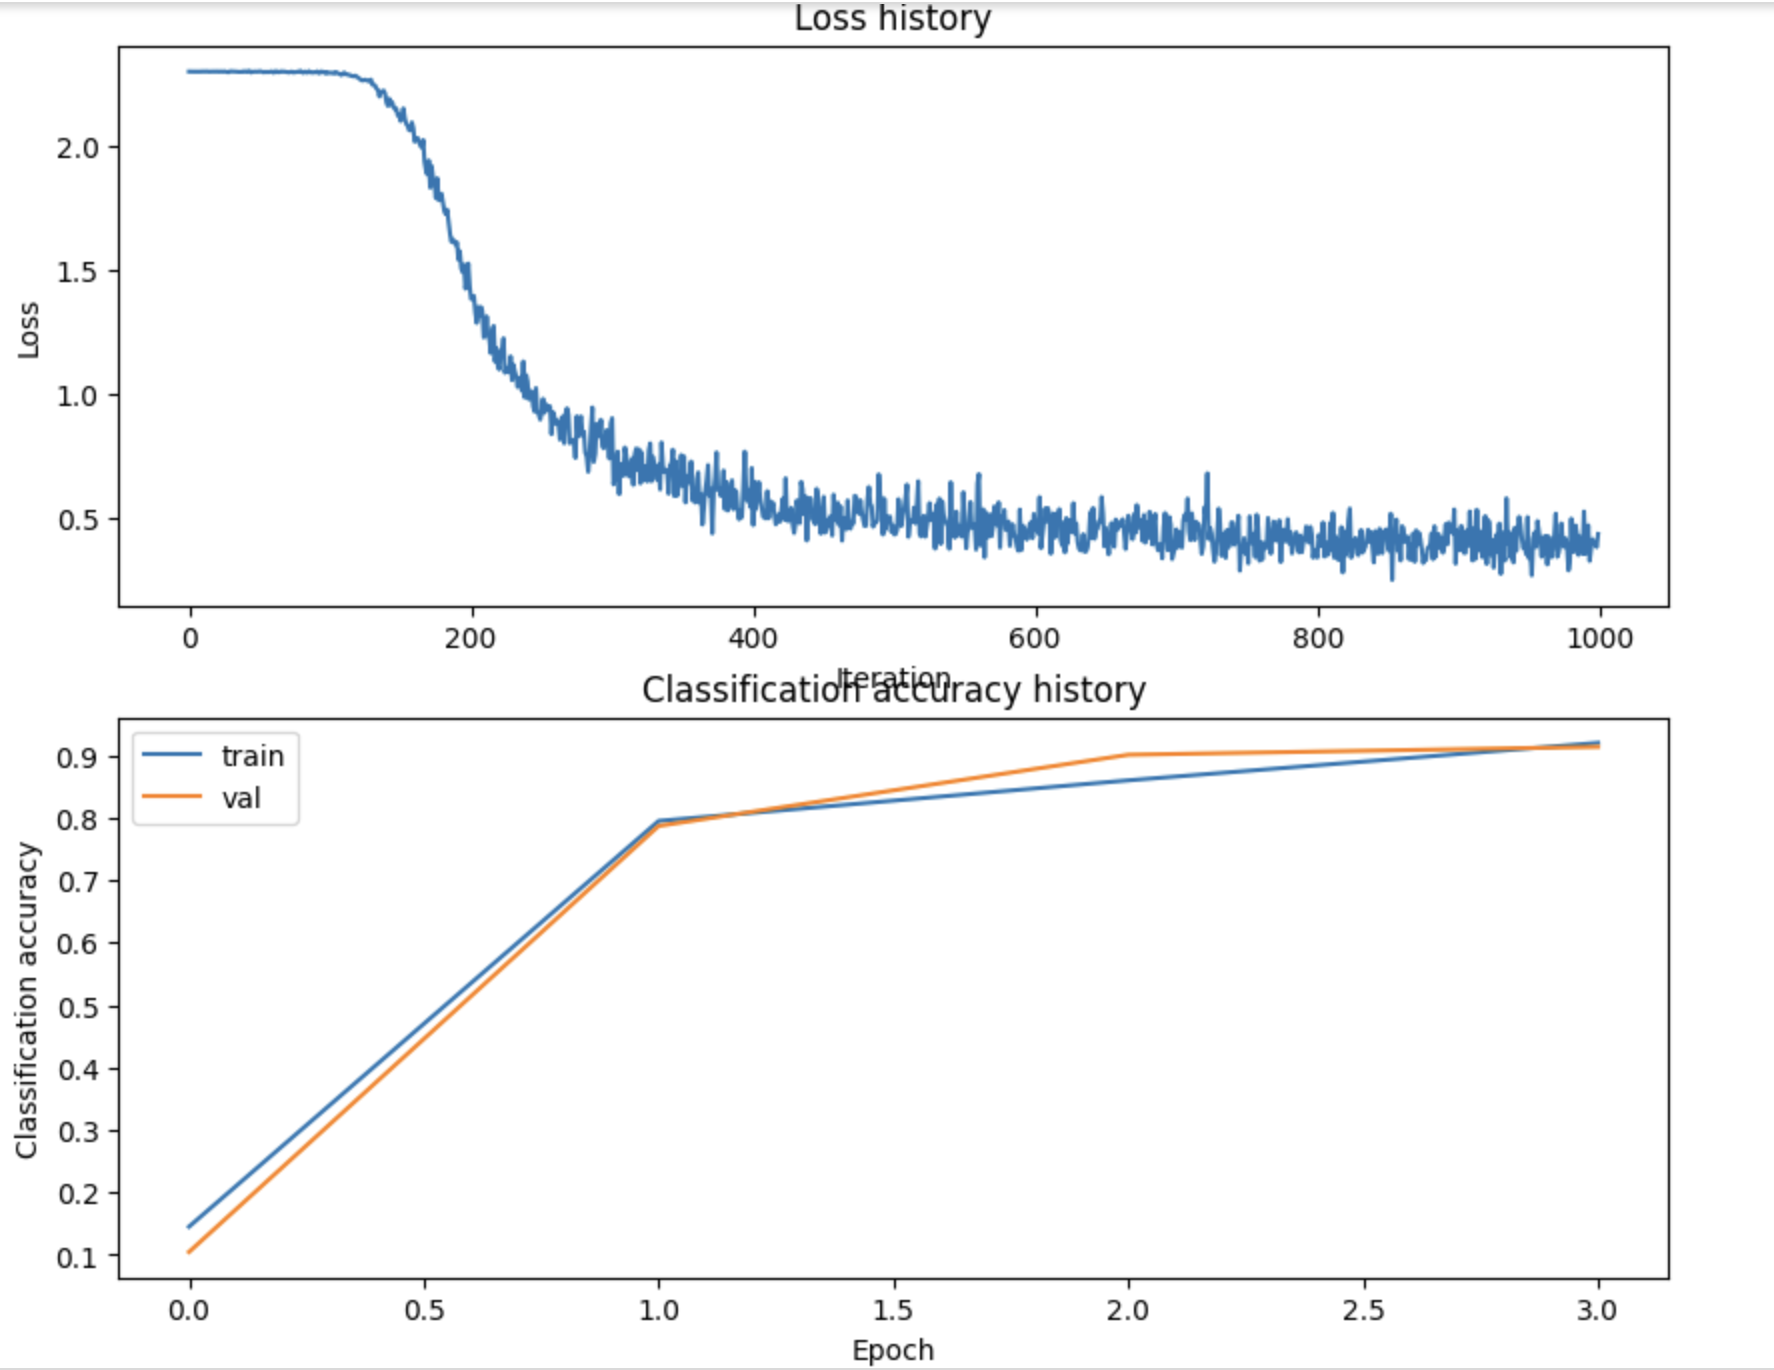
\includegraphics[width=0.8\linewidth]{loss_accuracy.png}
\caption{Loss history and Classification accuracy history}
\end{figure}

\begin{figure}[h]
\centering
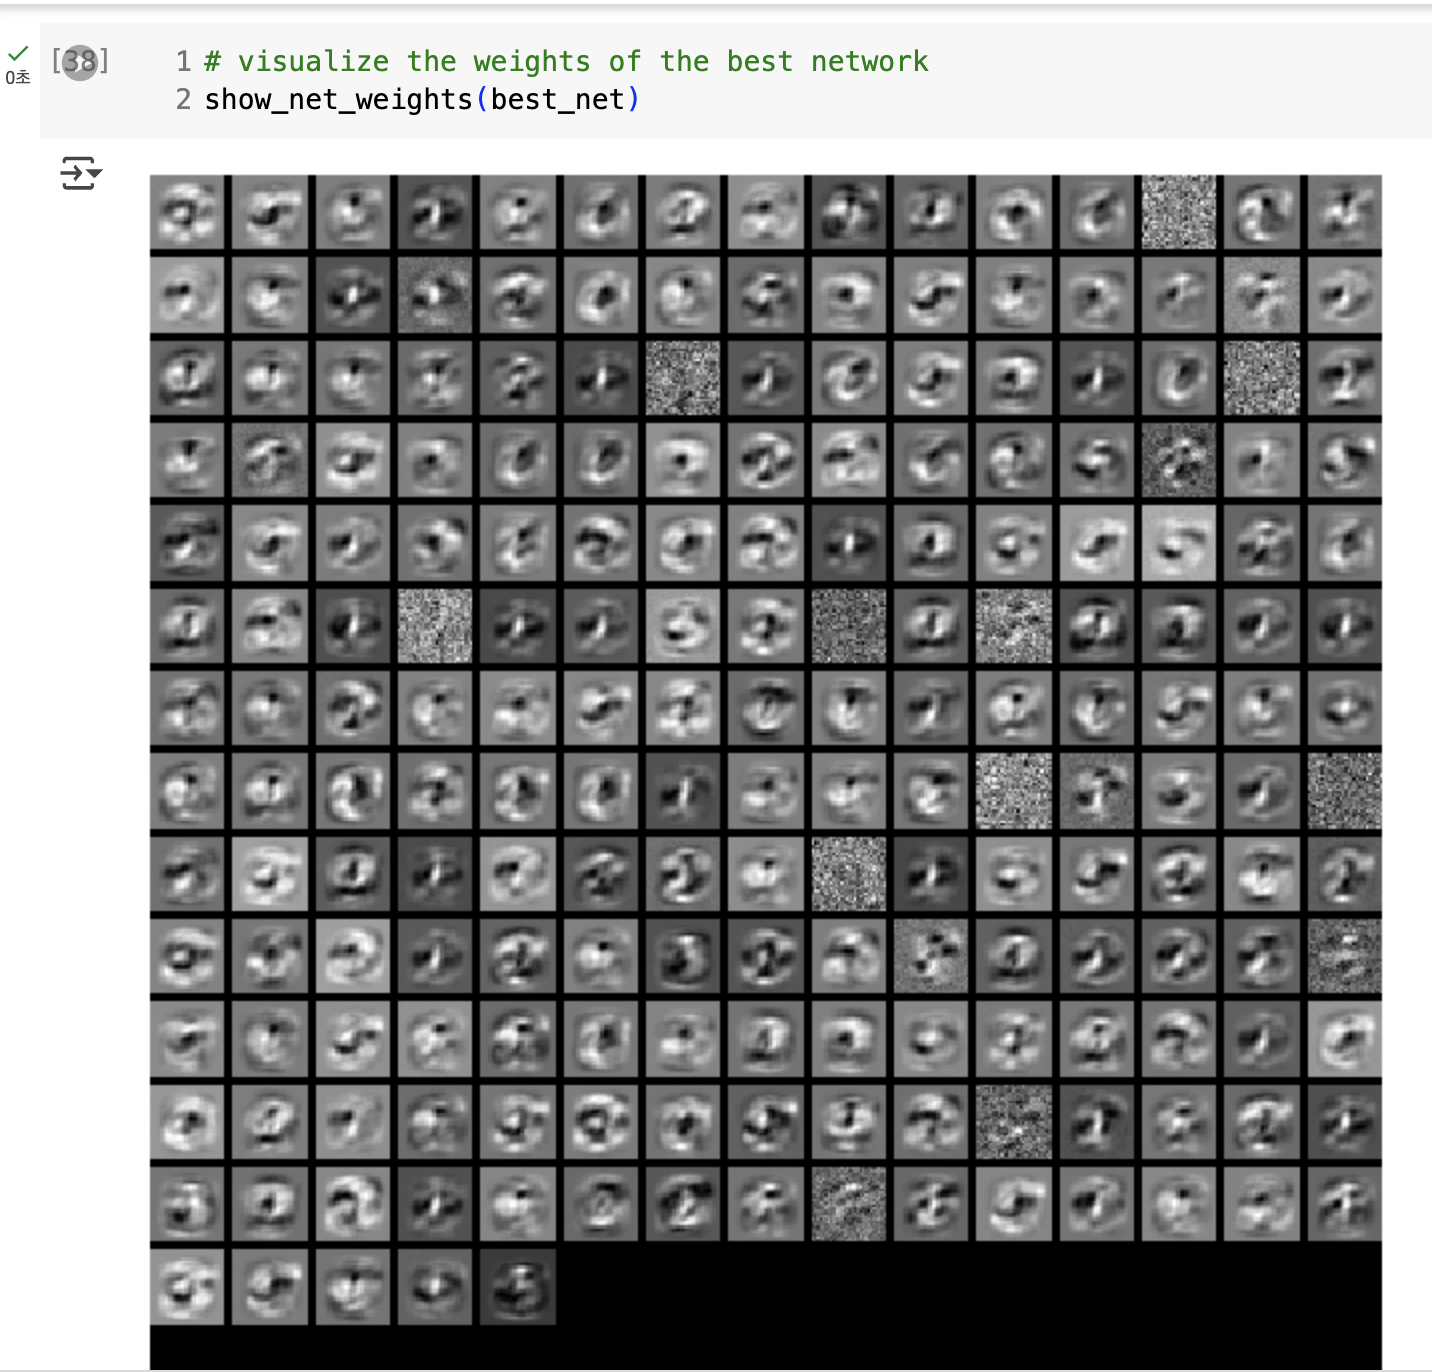
\includegraphics[width=0.8\linewidth]{show_net_weights.png}
\caption{Visualize the weights of the network}
\end{figure}

\begin{figure}[h]
\centering
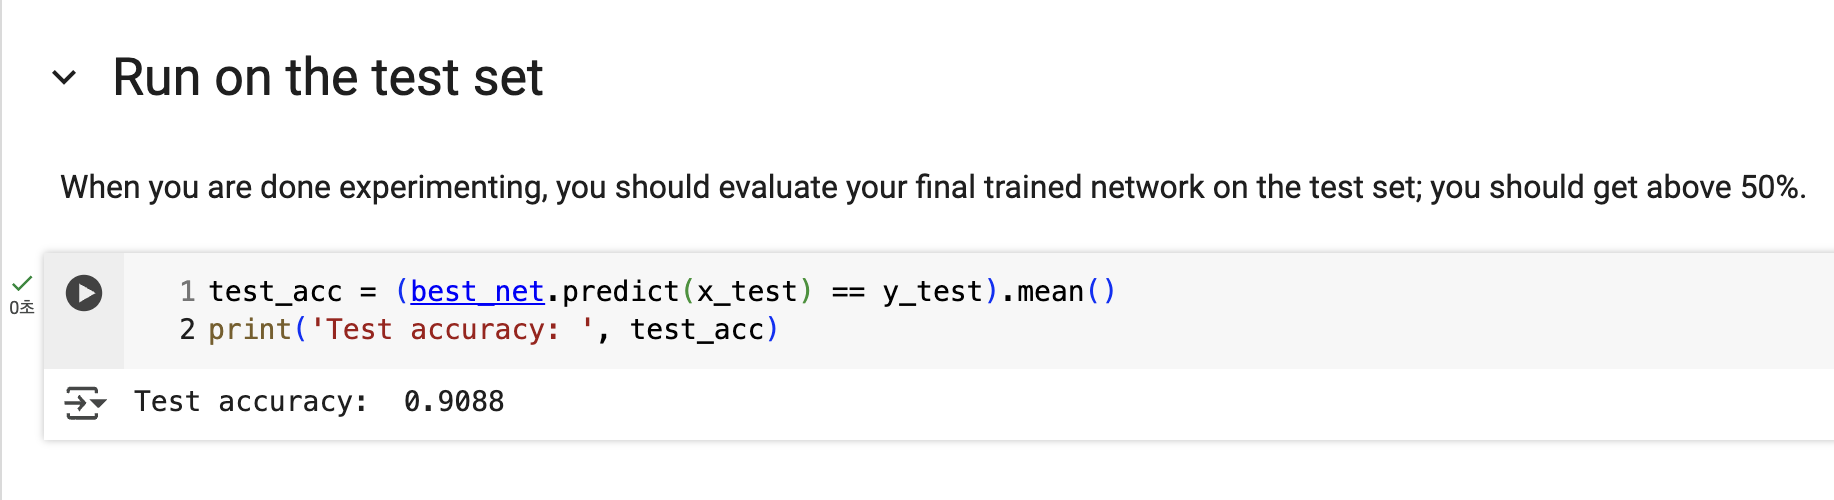
\includegraphics[width=0.8\linewidth]{test_accuracy.png}
\caption{Final test accuracy of 90.88\% achieved on the MNIST dataset.}
\end{figure}

\section{Discussion}
\label{sec:discussion}

The learning rate had a significant impact on convergence.
Small learning rates led to slow training, while large rates caused unstable updates.
We found that using a learning rate around $10^{-1}$ with regularization strength $10^{-3}$ gave the best results.

The hidden layer size also affected the model capacity. Larger hidden sizes increased accuracy but led to overfitting.
The validation accuracy tracked training accuracy well, indicating the model generalized properly with the chosen settings.

Our final model surpassed the target validation accuracy of 36\%, achieving over 90\%.

%\section{Final copy}

You must include your signed IEEE copyright release form when you submit your finished paper.
We MUST have this form before your paper can be published in the proceedings.

Please direct any questions to the production editor in charge of these proceedings at the IEEE Computer Society Press:
\url{https://www.computer.org/about/contact}.
{
    \small
    \bibliographystyle{ieeenat_fullname}
    \bibliography{main}
}

% WARNING: do not forget to delete the supplementary pages from your submission 
% \clearpage
\setcounter{page}{1}
\maketitlesupplementary


\section{Rationale}
\label{sec:rationale}
% 
Having the supplementary compiled together with the main paper means that:
% 
\begin{itemize}
\item The supplementary can back-reference sections of the main paper, for example, we can refer to \cref{sec:intro};
\item The main paper can forward reference sub-sections within the supplementary explicitly (e.g. referring to a particular experiment); 
\item When submitted to arXiv, the supplementary will already included at the end of the paper.
\end{itemize}
% 
To split the supplementary pages from the main paper, you can use \href{https://support.apple.com/en-ca/guide/preview/prvw11793/mac#:~:text=Delete%20a%20page%20from%20a,or%20choose%20Edit%20%3E%20Delete).}{Preview (on macOS)}, \href{https://www.adobe.com/acrobat/how-to/delete-pages-from-pdf.html#:~:text=Choose%20%E2%80%9CTools%E2%80%9D%20%3E%20%E2%80%9COrganize,or%20pages%20from%20the%20file.}{Adobe Acrobat} (on all OSs), as well as \href{https://superuser.com/questions/517986/is-it-possible-to-delete-some-pages-of-a-pdf-document}{command line tools}.

\end{document}
